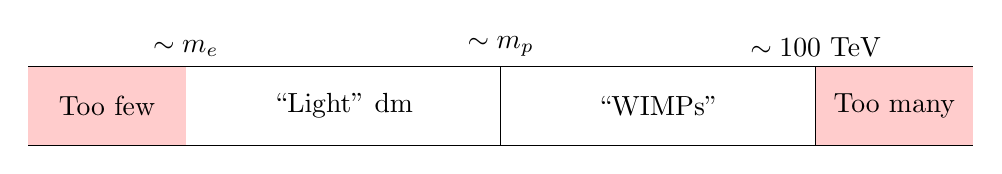
\begin{tikzpicture}
  % horizontal top/bottom lines
  \draw (0,0) -- (12,0);
  \draw (0,1) -- (12,1);
  % dividing lines along with relevant scale markers
  \draw (2,0) -- (2,1) node[above] {$\sim m_e$};
  \draw (6,0) -- (6,1) node[above] {$\sim m_p$};
  \draw (10,0) -- (10,1) node[above] {$\sim100~$TeV};
  % fill non-thermal ranges with light red
  \fill [red!20!white] (0,0) rectangle (2,1);
  \fill [red!20!white] (10,0) rectangle (12,1);
  % labels offering descriptions of ranges inside the boxes
  \node at (1,0.5) {Too few};
  \node at (4,0.5) {``Light'' \ac{dm}};
  \node at (8,0.5) {``WIMPs''};
  \node at (11,0.5) {Too many};
\end{tikzpicture}
